\section{Unweighted Graphs}
\subsection*{Types}
\resizebox{\linewidth}{!}{%
\begin{tikzpicture}[
    p/.style ={
        minimum size=5em,
        circle,
        white,
        fill=blue!60,
        draw=black
    }
    ]

    \node[p] (bob) {bob};
    \node () [above=1em of bob] {\large undirected \& unsigned};
    \node[p] (mark) [below=of bob] {mark};
    \node[p] (alice) [left=of mark] {alice};
    \node[p] (rob) [right=of mark] {rob};
    \node[p] (maria) [below=of mark] {maria};

    \foreach \src/ \dst in {bob/alice, rob/bob, mark/alice, rob/mark, alice/maria, rob/maria}
        \path[draw,thick] (\src) -- (\dst);
\end{tikzpicture}
\begin{tikzpicture}[
    p/.style ={
        minimum size=5em,
        circle,
        white,
        fill=blue!60,
        draw=black
    }
    ]

    \node[p] (bob) {bob};
    \node () [above=1em of bob] {\large directed};
    \node[p] (mark) [below=of bob] {mark};
    \node[p] (alice) [left=of mark] {alice};
    \node[p] (rob) [right=of mark] {rob};
    \node[p] (maria) [below=of mark] {maria};

    \foreach \src/ \dst in {bob/alice, rob/bob, mark/alice, rob/mark, alice/maria, rob/maria}
        \path[->,thick] (\src) edge (\dst);
\end{tikzpicture}
\begin{tikzpicture}[
    p/.style ={
        minimum size=5em,
        circle,
        white,
        fill=blue!60,
        draw=black
    },
    inside/.style ={
        midway,
        fill=white,
        inner sep=1.5pt,
        outer sep=2pt
    }
    ]

    \node[p] (bob) {bob};
    \node () [above=1em of bob] {\large weighted};
    \node[p] (mark) [below=of bob] {mark};
    \node[p] (alice) [left=of mark] {alice};
    \node[p] (rob) [right=of mark] {rob};
    \node[p] (maria) [below=of mark] {maria};

    \foreach \src/ \dst/ \weight in {bob/alice/1, rob/bob/0.75, mark/alice/0.5, rob/mark/0.5, alice/maria/0.75, rob/maria/1}
        \draw[draw,thick] (\src) -- node[inside] {\weight} (\dst);
\end{tikzpicture}
}

\subsection*{Depth First Search}
Search down a path from a vertex as far as you can go. Then backtrack to the last vertex from which a different path could have been taken. $O(V+E)$

\subsection*{Breadth First Search}
Search all the paths at a uniform depth from the source before moving into deeper paths.

\subsection*{Topological Sort}
Can find a top.\ ord.\ in $O(V+E)$ time.

\subsubsection*{Topological Ordering}
An ordering of the nodes in a directed graph where for each directed edge from node A to node B,
node A appears before node B in the ordering.

Top.\ ords.\ are NOT unique.

%\vspace{1em}! % Fixes clipping issue with "Top. ..." text

%\newcolumn
A graph which contains a cycle cannot have a valid ordering:

\resizebox{.5\linewidth}{!}{%
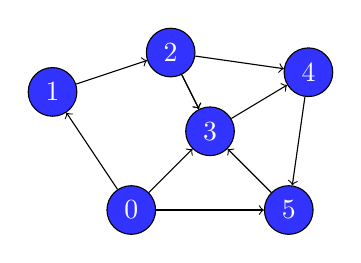
\begin{tikzpicture}[
    n/.style ={
        circle,
        white,
        fill=blue!80,
        draw=black
    }
    ]
    \foreach \x/ \pos in {{0/(1,0)}, {1/(0,1.5)}, {2/(1.5,2)}, {3/(2,1)}, {4/(3.25,1.75)}, {5/(3,0)}}
        \node[n] (\x) at \pos {\x};

    \foreach \src/ \dst in {0/1, 1/2, 2/3, 0/3, 0/5, 3/4, 2/3, 2/4, 4/5, 5/3}
        \draw[->] (\src) -- (\dst);

\end{tikzpicture}
}

The only type of graph which has a valid top.\ ordering is a {\bfseries Directed Acyclic Graph (DAG)}.
These are graphs with directed edges and no cycles.

ie: Program dependency graph.

\resizebox{\linewidth}{!}{%
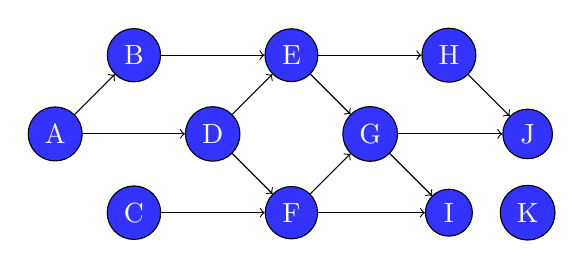
\begin{tikzpicture}[
    n/.style ={
        circle,
        white,
        fill=blue!80,
        draw=black
    }
    ]
    \foreach \x/ \pos in {{A/(0,1)}, {B/(1,2)}, {C/(1,0)}, {D/(2,1)}, {E/(3,2)},
                          {F/(3,0)}, {G/(4,1)}, {H/(5,2)}, {I/(5,0)}, {J/(6,1)},
                          {K/(6,0)}}
        \node[n] (\x) at \pos {\x};

    \foreach \src/ \dst in {A/B, A/D, B/E, D/E, D/F, C/F, E/G, E/H, F/G, F/I, G/I, G/J, H/J}
        \draw[->] (\src) -- (\dst);

\end{tikzpicture}
}

\subsubsection*{Topological Algorithm}
\begin{enumerate}
    \item Pick an unvisited node
    \item Beginning w/ the selected node, do a DFS exploring only unvisited nodes.
    \item On the recursive callback of the DFS, add the current node to the top.\ ordering in rev.\ order.
\end{enumerate}

